\subsubsection{Navigation}
Our original approach was to search the panel by using long range laser sensor.
However, it was found to be difficult to detect the panel at a distance because of the low density of points provided by the sensor.
Therefore, we use a second approach where the robot navigates around the arena and searches for the panel using pointcloud data from its stereo camera.
Initially, if the panel is not visible within the robot's field of view, meaning that the panel is either out of range of the camera or is in another direction, the robot will navigate around the arena to search for the panel.
Then, when the panel enters the sensing range of the stereo camera, the robot recognizes the panel by finding
the cluster of pointcloud that sits approximately 1 meter above the ground (Fig.\ref{fig: task2_panel-recognition}) and approaches the panel.
Finally, the robot circles around the panel to recognize its front side, then move to position itself in front of the panel.

\begin{figure}[htb]
  \begin{center}
    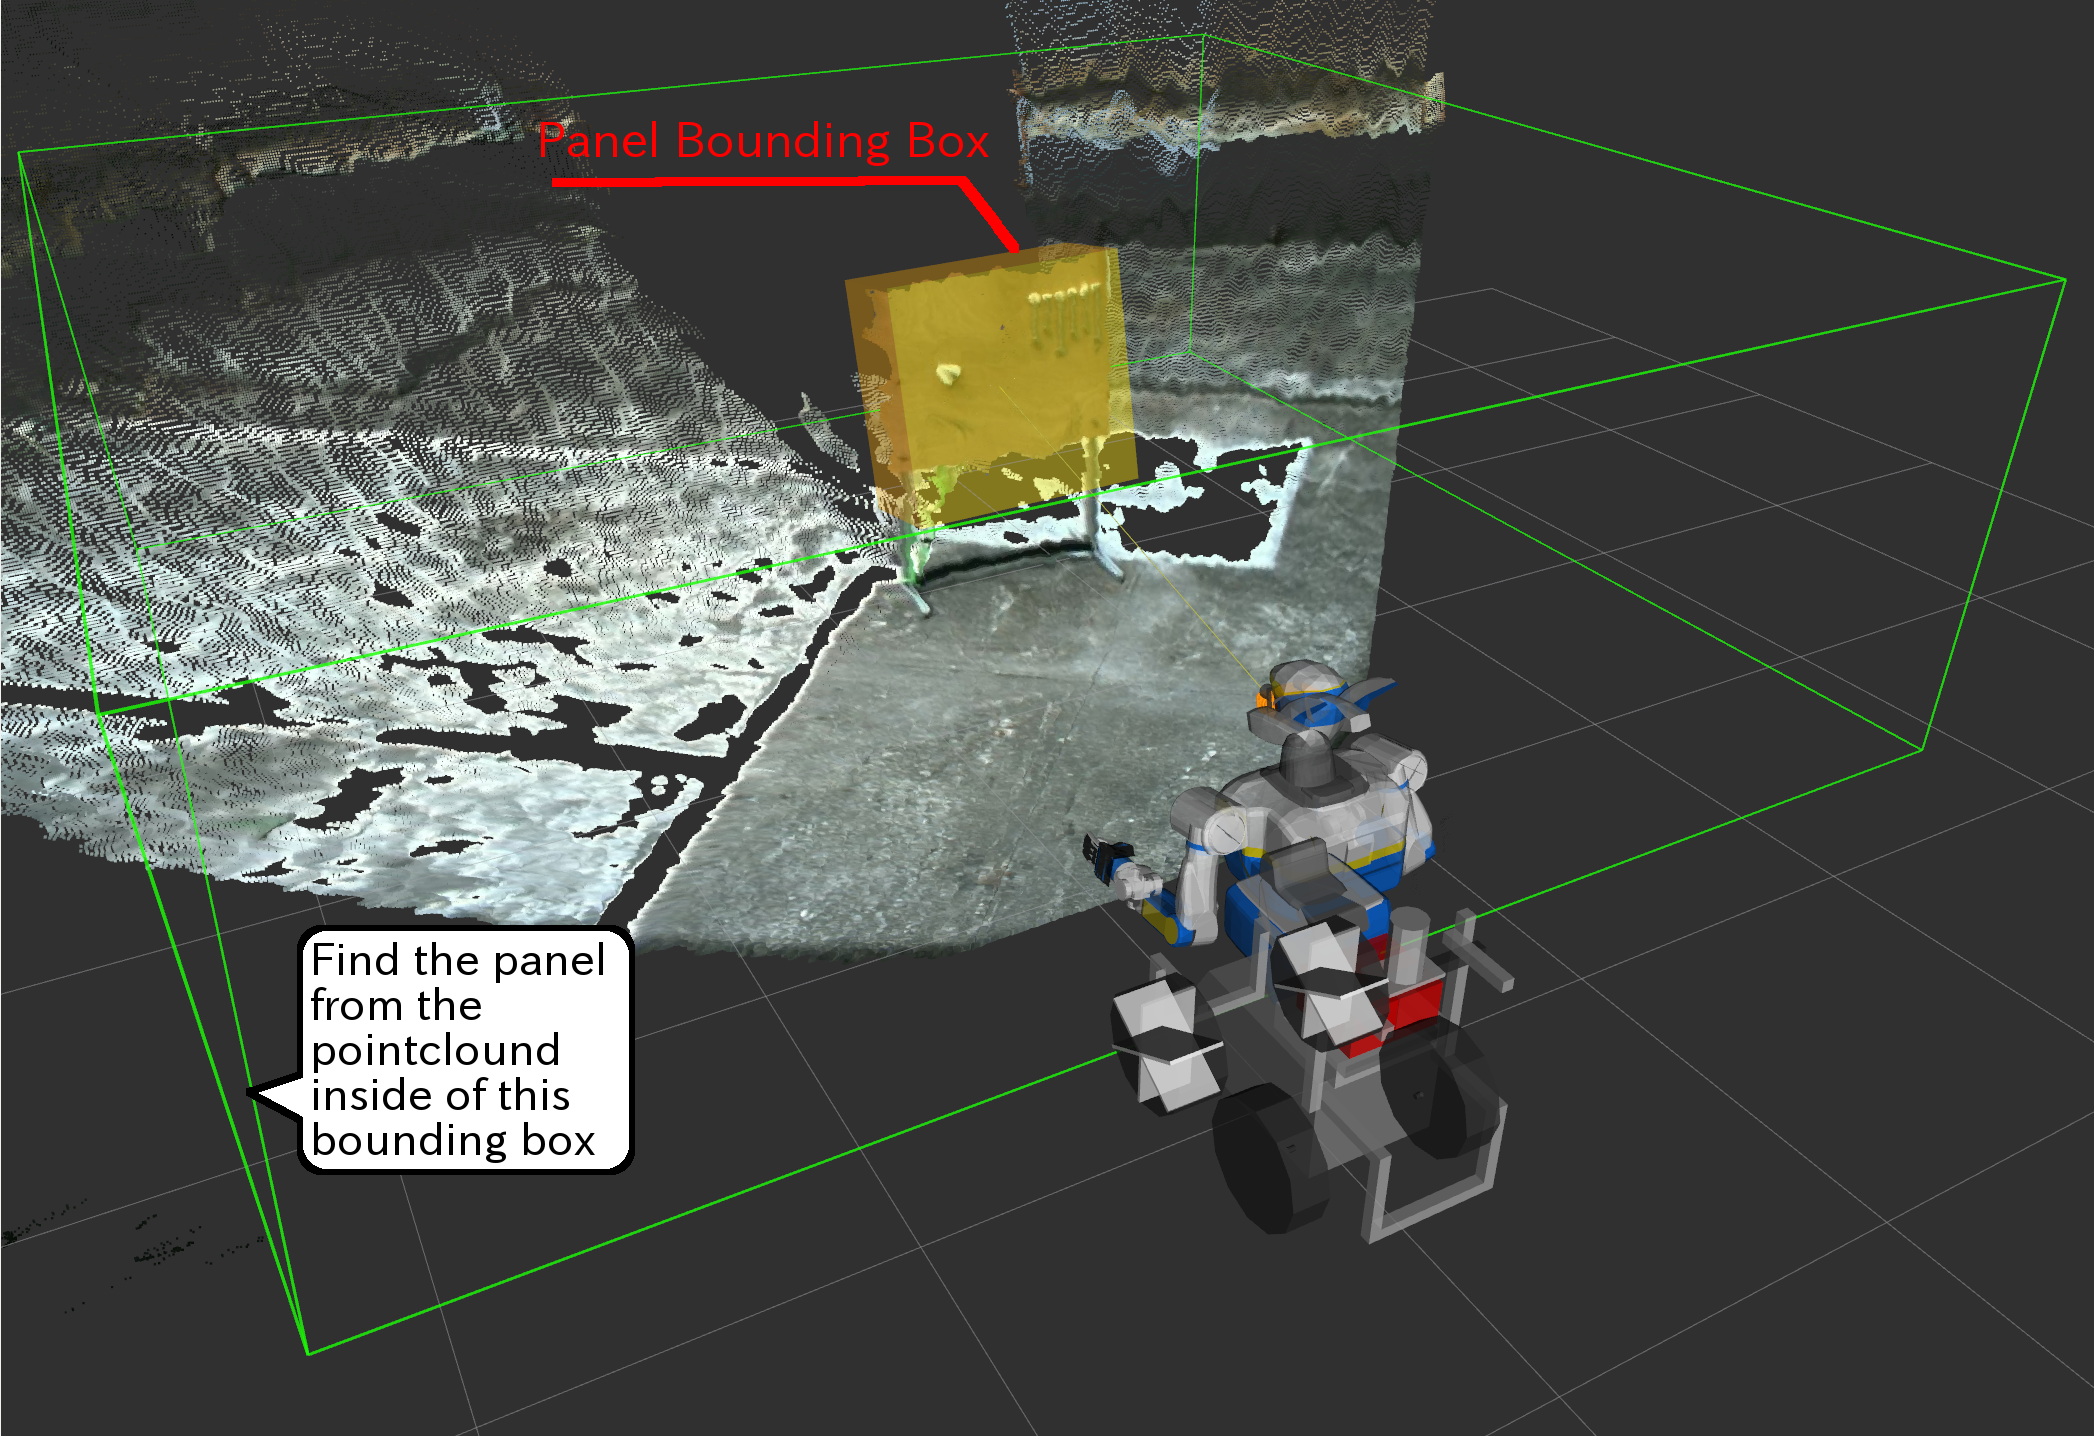
\includegraphics[width=0.80\columnwidth]{sections/task2/images/panel_detect.png}
    \caption{Panel Recognition from Pointcloud}
    \label{fig: task2_panel-recognition}
  \end{center}
\end{figure}

\subsubsection{Wrench and Valve Stem Recognition}
We detected the wrenches and valve stem by manually selecting an ROI in our previous progress report, and we were able to recognize
the length of the wrenches, and the position of the wrenches and the valve stem.

Our next target is autonomous recognition and recognition of the orientation of the panel relative to the robot.
We achieve this by first fitting a plane to the cloud points that is in front of the robot, and then finding the upper-right corner of the plane and calculating its orientation.
The position of the wrenches and valve stem on the panel is fixed and known, so we can easily determine the position and orientaiton of them once we have detected the panel (Fig.\ref{fig: task2_object-recognition}).

We tested the recognition method described above and confirmed that the accuracy of the recognition is good enough for carrying out the task.

\begin{figure}[htb]
  \begin{center}
    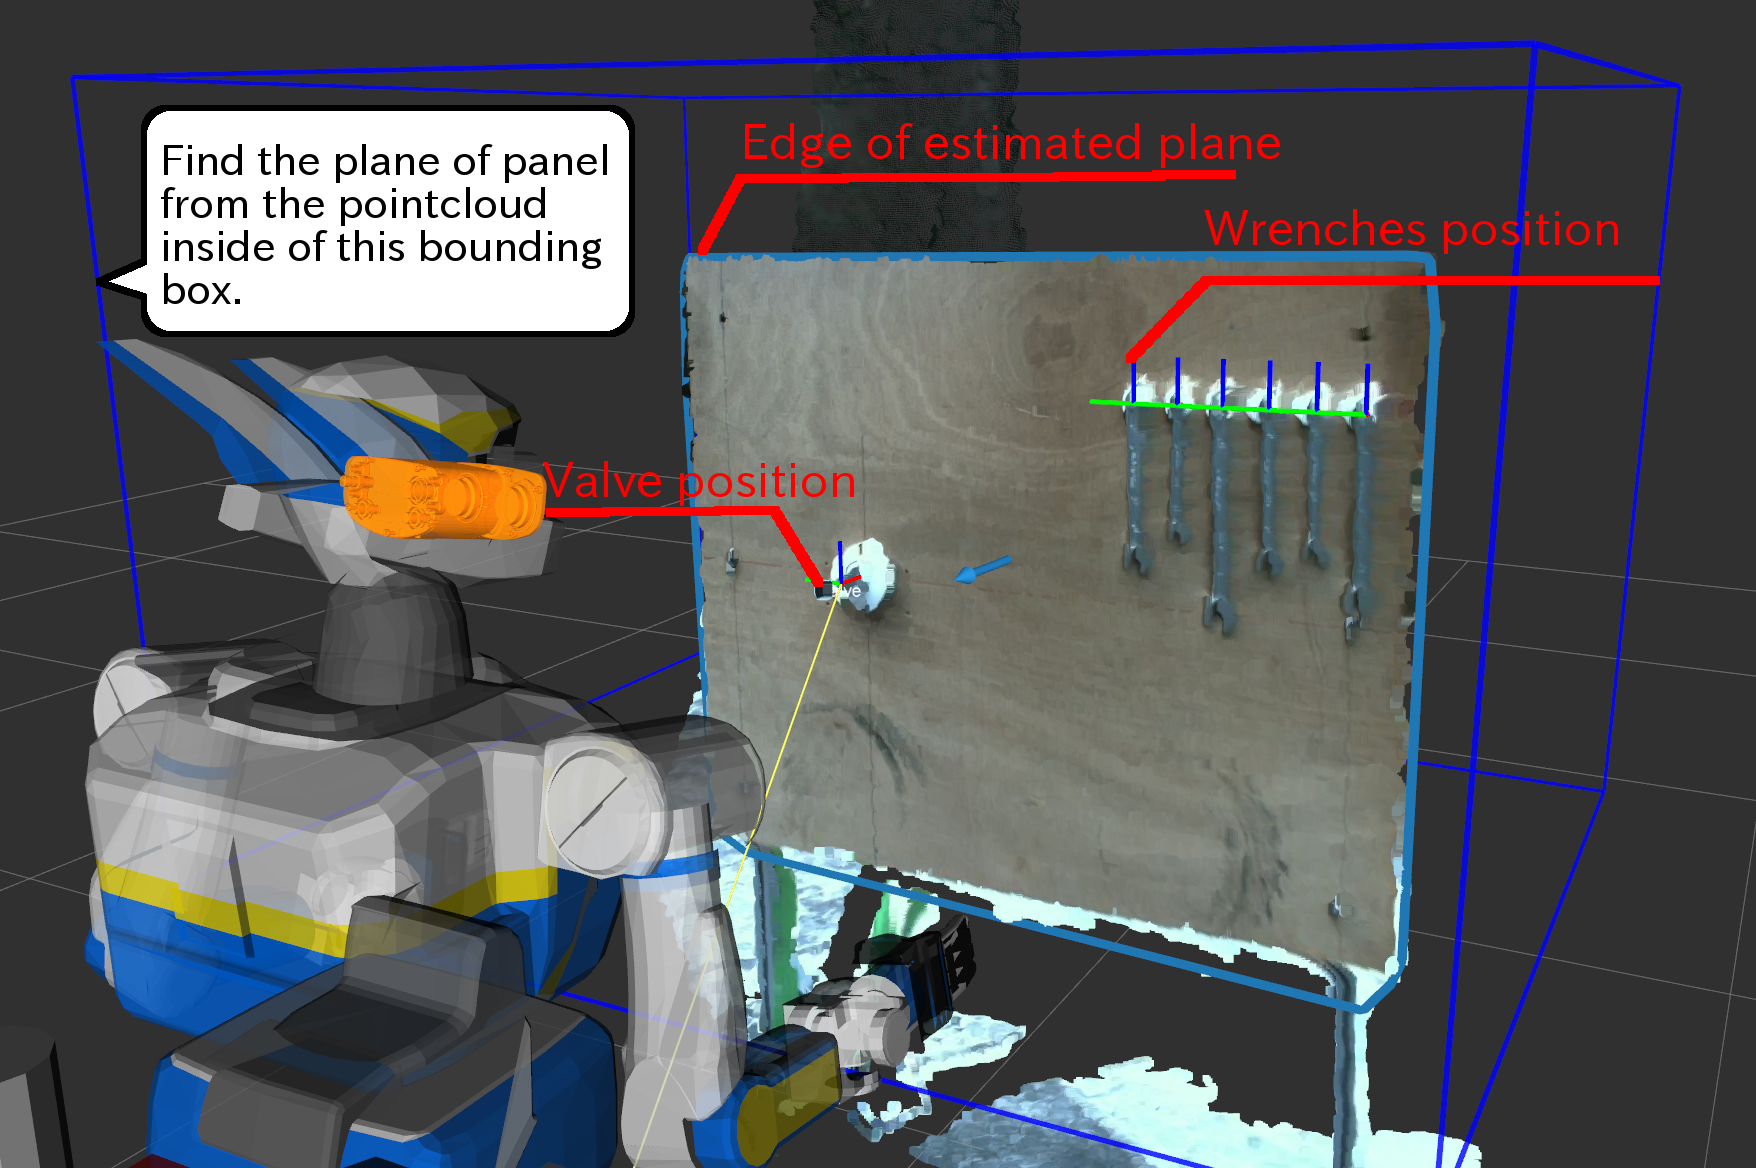
\includegraphics[width=0.80\columnwidth]{sections/task2/images/wrench_valve_recog.png}
    \caption{Wrench and Valve Stem Recognition}
    \label{fig: task2_object-recognition}
  \end{center}
\end{figure}

\subsubsection{Wrench Picking}
We accomplished wrench picking by simply positioning the gripper to the detected wrench's position.

In order to improve the success rate, we will be incorporating the use of a handeye camera and visual feedback control.


\subsubsection{Wrench Fitting and Turning}
We have accomplished wrench fitting and turning in our previous report, and we will be using handeye visual feedback control to improve it performance as well.
